\documentclass[document.tex]{subfiles}
\begin{document}
\section*{Exercise 1:}

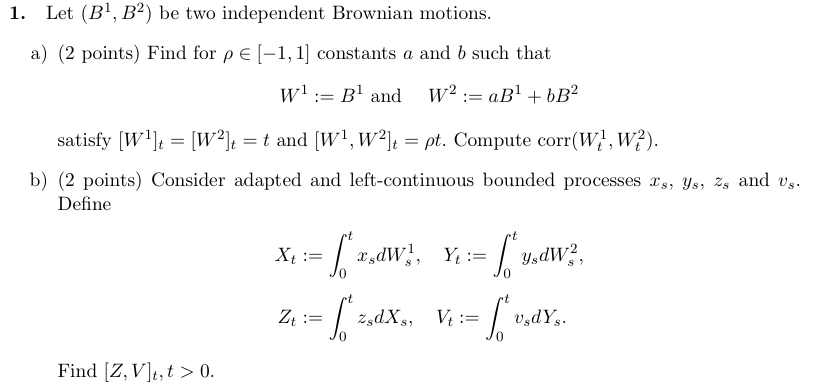
\includegraphics[width=\textwidth]{ex1.png}

\subsection*{a)}
\begin{align*}
	\rho t &= \qcVar{W^1}{W^2} \\
	&= \qcVar{B^1}{a B^1 + b B^2} \\
	&\text{, since the quadratic covariation is bilinear in it's arguments}\\
	&= a \qcVar{B^1}{B^1} + b \underbrace{\qcVar{B^1}{B^2}}_{=0, \text{since} B^1 \text{and} B^2 \text{independent}} \\
	&= a \qVar{B^1} \\
	&= a t \\
\Rightarrow a &= \rho	 
\end{align*}


\end{document}
